\chapter{Réalisation et résultats}
\section{Introduction}

\section{Environnement de développement}
Dans cette section nous allons présenter les différents outils (logiciels et matériels) qui ont été utilisé pour l'implémentation de BETHANO.
	\subsection{Machines utilisées}
	\paragraph{}
	Principalement, le développement se divise en deux parties : 
	\begin{itemize}
		\item Apprentissage : les données sont récoltées ou construites puis nettoyées et préparées. Les modèles sont développés, entraînés puis testés.
		\item Les modules sont implémentés puis connectés et intégrés dans l'application.
	\end{itemize}
	\par Pour ce faire nous avons utilisé des machines dont les spécificités sont mentionnés ci-dessous :
	%TODO insert figures with their caption here OR one diagram with specs
	\begin{figure}[H] 
		\centering
		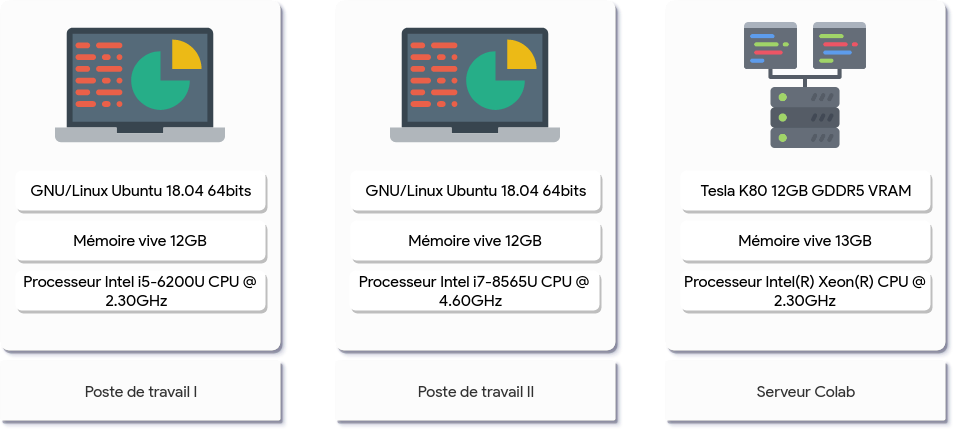
\includegraphics[width=0.88\linewidth]{images/implementation/machines.png}
		\caption{Caractéristiques des machines}
		\label{fig:machines}
		
	\end{figure}
	\par
	En ce qui concerne la partie logicielle une liste non exhaustive est présentée ci dessous, qui ne mentionne que les outils les plus utilisés et les plus exploités :
	\subsection{Langages de programmation}
		\begin{figure}[H] 
		\centering
		
\includegraphics[width=0.3\linewidth]{images/implementation/langs.png}
		\caption{Langages de programmation utilisés}
		\label{fig:langs}
	\end{figure}
		\subsubsection*{Python}
		\label{python}
		\paragraph{}
		 C'est un langage de programmation interprété de haut niveau, structuré et open source. Il est multi-paradigme (orienté objet, programmation fonctionnelle et impérative) et multi-usage. Il est, comme la plupart des applications et outils open source, maintenu par une équipe de développeurs un peu partout dans le monde. Il offre une grande panoplie d'extensions (packages) pour résoudre une variété de problèmes, qu'ils soient reliés au développement d'applications de bureau, web ou mobiles \cite{python}.
		
		\subsubsection*{Javascript} 
		\paragraph{}
		JavaScript est un langage de programmation utilisé principalement par les navigateurs web pour exécuter un bout de code incorporé dans une page web plus communément appelé script. Il permet la manipulation de tout les éléments inclus dans une page, et par conséquent permet une gestion dynamique de ces dernier. Il est beaucoup utilisé du coté client mais peut aussi être exécuté du coté serveur. Tout comme Python il offre une grande variété dans le choix des modules qui peuvent ajouter de nouvelles fonctionnalités, le tout géré par un gestionnaire de module \textit{npm} \footnote{Node Package Manager ou Gestionnaire de packages Node} devenu un standard \cite{js}.
	
	\subsection{Librairies et bibliothèques}
	\begin{figure}[H] 
		\centering
		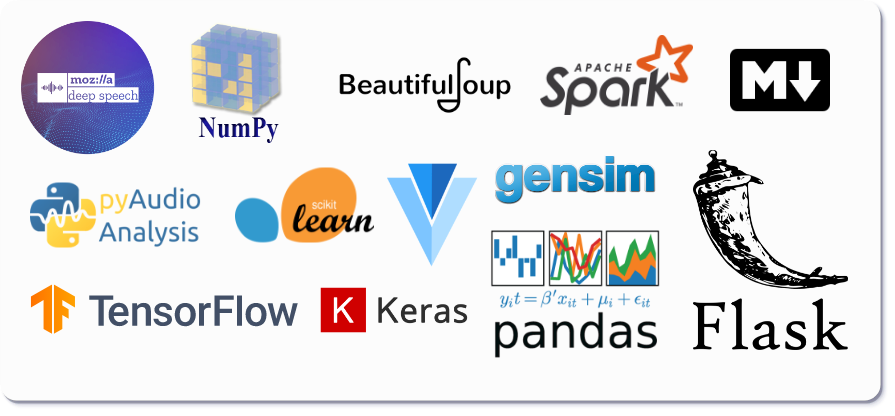
\includegraphics[width=0.9\linewidth]{images/implementation/libs_frams.png}
		\caption{Bibliothèques et librairies les plus utilisées}
		\label{fig:libs_frams}
	\end{figure}
		\subsubsection*{DeepSpeech API}
		\paragraph{}
		Package python qui fait office d'interface entre un script Python et la librairie de reconnaissance automatique de la parole DeepSpeech \cite{deepspeech_paper}. Il permet entre autre de charger différents modèles acoustiques ou modèles de langues. Il offre aussi la possibilité d'utiliser des scripts d'apprentissage prédéfinis pour peu que les données soient organisé suivant une certaine norme, ces scripts sont notamment hautement paramétrables \cite{deepseech_github}.
		
		\subsubsection*{PyAudio}
		\paragraph{}
		Librairie python destinée à la manipulation des fichiers ou flux audios. Elle offre entre autre la possibilité d'extraire des méta-données sur un flux audio (fréquence d'échantillonnage, débit ...). La possibilité d'extraire le vecteur de caractéristiques d'un extrait audio est aussi présente comme fonctionnalité \cite{pyaudio}.
		
		\subsubsection*{Beatiful Soup}
		\paragraph{}
		Bibliothèque Open source permettant l'analyse de fichier html pour en extraire ou y injecter des données. Principalement utilisée pour filtrer les balises nécessaire depuis une page web \cite{bs4}.
		
		\subsubsection*{PySpark}
		\paragraph{}
		Package Python utilisé comme interface pour interagir avec un serveur Spark. Il permet entre autre de lire et écrire des données dans le nouveau format Hadoop \cite{pyspark}.
		
		\subsubsection*{Scikit-Learn}
		\paragraph{}
		Bibliothèque Open source conçue pour rapidement développer des modèles pour l'apprentissage automatique, principalement utilisé pour ses nombreux outils de pré-traitement des données (codification, normalisation, filtrage ...) \cite{sklearn}.
		
		\subsubsection*{Numpy}
		\paragraph{}
		Bibliothèque spécialisée dans la manipulation de grands volumes de données numériques, notamment les vecteurs (tableaux) multi-dimensionnels, les opérations sur ces dernier sont implémentés en C pour optimiser au maximum leur coût en temps de calcul ou ressources mémoires utilisées. Elle offre des structures de données compatibles avec beaucoup d'autre librairies comme Tensorflow ou Keras \cite{numpy}.
		
		\subsubsection*{Tensorflow \& Keras}\label{tf&keras}
		\paragraph{}
		Vaste librairie dédiée à l'apprentissage automatique, et plus particulièrement au réseaux de neurones et l'apprentissage profond. Optimisée pour exécuter des opérations à grande échelle et massivement distribuées sur un réseau, Tensorflow offre la possibilité d'implémenter une grande variété d'architectures de modèles avec un maximum d'efficacité. Elle dispose d'un package Python permettant d'interagir avec le cœur de la librairie mais reste néanmoins assez bas-niveau et rudimentaire. Keras quant à lui propose de rajouter une couche d'abstraction à Tensorflow. c'est une package python destiné à faciliter le développement de modèles pour l'apprentissage profond tout en offrant la possibilité de rajouter et modifier un grand nombre de fonctionnalités par défaut. Sa force réside dans le fait qu'il peut utiliser au plus bas niveau plusieurs librairies autre que Tensorflow comme Theano et CNLTK \cite{tf,keras,theano,cnltk}.
		
		\subsubsection*{Flask}
		\paragraph{}
		Micro-librairie Open source dédiée au développement d'applications basé web. De base, cette librairie est très légère, mais elle offre la possibilité d'ajouter des extensions qui s'intègrent très facilement au système de base \cite{flask}.
		
		\subsubsection*{Vuetify}
		\paragraph{}
		Librairie Open source basée sur VueJs dédié au développement d'interface web ou mobile. Elle implémente le paradigme Material Design de Google et offre la possibilité d'étendre les composants de base et de créer des interfaces belle et adaptatives \cite{vuetify}.
	\subsection{Outils et logiciels de développement}
		\subsubsection*{PyCharm}
		\paragraph{}
		PyCharm est un environnement de développement intégré spécialisé et optimisé pour programmer dans le langage Python (voir \ref{python} ci dessus). Il permet l'analyse de code en continue et offre un débogueur intégré pour exécuter un code instruction par instruction. Il offre également l'intégration de logiciel de gestion de versions comme Git \cite{git}, et supporte le développement web avec Django et Flask \cite{pycharm}.
		
		\subsubsection*{Git}
		\paragraph{}
		Système de gestion de versions décentralisé. Il permet entre autre de gérer les différentes versions d'un projet durant son développement, mais aussi de garder l'historiques des modifications effectuées ainsi que la possibilité de régler des conflits lors de l'intégration finale des contributions des développeurs \cite{Git}.
		
		\subsubsection*{Google Colaboratory}
		\paragraph{}
		Colaboratory est un outil de recherche et développement pour la formation et la recherche associées à l'apprentissage profond. C'est un environnement Python qui ne nécessite aucune configuration et offre la possibilité d'utiliser de puissantes machines rendues accessibles par Google pour accélérer la phase d'apprentissage \cite{colab}.
		
		\subsubsection*{Protégé}
		\paragraph{}
		Protégé est un système dédié à la création et la modification d'ontologies. Il est développé en Java et est Open source distribué sous une licence libre (la Mozilla Public License). Il se démarque par le fait qu'il permet de travailler sur des ontologies de très grandes dimensions 
		\cite{protege}.
		
		
\section{ASR (to be changed)}
\paragraph{}
Pour ce premier module, il a été très difficile d'effectuer les tests idéals. En effet, nous n'avons pas pu trouver un ensemble de données qui proposait du contenu en rapport avec Bethano. Cependant puisque nous avons pu construire un mini-ensemble pour tester l'apport de notre modèle de langue. Les résultats ne doivent pas être pris comme une référence absolue, mais plutôt comme une indication pour de futurs possible tests.
	\subsection{Ensemble de test}
	\paragraph{}
	Pour tester le modèle acoustiques, les données récoltées à travers le projet CommonVoice \ref{common_voice} constituent un assez bon échantillon. De par la nature des enregistrement (sur téléphone portable, par plusieurs genre et accent de locuteurs ...) et mais aussi de par le volume (environs 500 heures d'enregistrements audios). 
	\par
	Pour le modèle de langue il s'agit de celui mentionné dans la section \ref{lm}. Quelques modifications ont été rajoutée comme le filtrage des mots qui n'appartiennent pas à la langue anglaise. Mais au prix du sacrifice de quelques noms propres non reconnus ou bien de séquences de mots/lettres sans réel sens.
	\subsection{Méthodologie d'évaluation}
	\paragraph{}
	Les tests ont été effectués dans un serveur Colab pour libérer les machines locales. Les principales étapes sont les suivantes :  
	\begin{enumerate}
		\item \textbf{Préparation des données} : Les données sont téléchargé depuis le serveur de Mozilla pour être stockées sur le serveur. il faut ensuite lancer le script d'évaluation qui converti les fichiers audio en .wav et construit un fichier index au format .csv pour trouver les enregistrements sur le disque.
		\item \textbf{Métriques retenues} : À chaque lot de données (fixé à 64 instances) le \textbf{WER} (Word Error Rate) est calculé. Pour rappel la formule du WER est la suivante :
		\begin{equation*}
			WER(y,\hat{y}) = \frac{S+D+I}{S+D+C} = \frac{S+D+I}{N}
		\end{equation*}
		Où : 
		\begin{itemize}
			\item $y$ est la séquence de mots prédite appelée Hypothèse.
			\item $\hat{y}$ est la séquence de mots réelle appelée Référence.
			\item $S$ est le nombre de substituions (compté en mots) réalisées entre l'hypothèse et la référence.
			\item $D$ est le nombre de suppressions qu'a effectué le système. donc le nombre de mots supprimés dans l'hypothèse par rapport à la référence.
			\item $I$ est le nombre d'insertions effectuées par le système (c.à.d) le nombre de mots rajouté à l'hypothèse par rapport à la référence.
			\item $C$ est le nombre de mots bien placés.
			\item $N$ est la longueur totale de la séquence en nombre de mots
		\end{itemize}
		\item \textbf{Boucle d'évaluation} l'opération précédente est réitérée en incrémentant à chaque fois le taux d'utilisation de notre modèle de langue (de 20\% à 100\% avec un pas de 10\%). Le WER associé est ensuite comparé à celui obtenu en utilisant le modèle de langue par défaut que propose DeepSpeech. L'algorithme suivant explique les démarches :
%		TODO make algo here
	\end{enumerate}
	\subsection{Résultats}
	\paragraph{}
	Les résultats sont décrits dans les tableaux ... et ...
	\subsection{Intégration dans l'application}

\section{NLU (to be changed)}
\paragraph{}
Pour ce module, une approche assez classique à été utilisée, l'ensemble de test est extrait de l'ensemble d'apprentissage (plus de détail dans la section suivante ). Les métriques d'évaluation utilisées sont mentionnées dans la sous section \ref{nlu_steps}. Nous commençons d'abord par détailler le contenu de l'ensemble de tests. Puis nous présenterons la méthodologie suivie pour la réalisation de ces tests. Un tableau récapitulatif sera présenté avant la fin pour illustrer les différents résultats.
	\subsection{Ensemble de test}
	\paragraph{}
	Comme mentionné dans la section XXX, nous avons nous même construit un ensemble d'apprentissage relativement varié. Il regroupe essentiellement des commandes ou requêtes liées à l'exploration de fichier pour le moment car c'est la tâche rudimentaire que Bethano peut accomplir.
	\par
	L'ensemble de test est dérivé de celui d'apprentissage selon une politique de découpage basée sur le taux de présence d'un intent (intention). Comme illustré dans XXX, un pourcentage de chaque groupe d'instance affilié à la même classe est utilisé à la fois pour la validation et pour le test.
	
	Une liste exhaustive des intentions et slots est introduite respectivement dans les tableax XXX et XXX ci dessous :
%	TODO insert table of intents and their tags
%	TODO figure here for ratio splitting  
	\subsection{Méthodologie d'évaluation}
	\label{nlu_steps}
	\paragraph{}
	Après avoir construit l'ensemble de test, un parcours exhaustif des différentes combinaisons des paramètres suivant est effectué : 
	\begin{itemize}
		\item \textbf{Architecture d'encodage} :
		C'est à dire l'utilisation ou pas d'un réseau récurent LSTM de base ou bien BiLSTM. Le but étant de montrer que le modèle pourra mieux interprété les données en entrée s'il capture le contexte de chaque mots.
		
		\item \textbf{Nombre neurones pour la couche de classification d'intention } : Lorsque l'encodeur retourne le dernier vecteur d'état caché, ce dernier passera par un réseau de neurones complètement connecté et multi-couche (nombre de couches fixé à 3 par soucis de performance, une couche d'entrée, une couche intermédiera et une couche de sortie). Le nombre de neurones dans la couche caché dépend grandement de la complexité de la tâche à effectuer. La classification d'intentions pour l'exploration de fichier était relativement simple, nous avons commencé avec 32 neurones puis nous avons doublé ce nombre jusqu'à 512 pour, en théorie, donnée plus de puissance au classificateur tout en évitant une sur-apprentissage par surplus de neurones.
		
		\item \textbf{Nombre d'unités d'une cellule LSTM (respectivement BiLSTM)}:
		Comme mentionné dans XXXXX, les portes d'une cellule LSTM (résp. BiLSTM) sont en vérité des réseaux de neurones denses (complètement connectés) et donc un ensemble de matrice de poids à être optimiser. La capacité à "apprendre" la représentation des séquence dépend donc aussi du nombre de neurones dans ces mini-réseaux. Par le même raisonnement employé pour le classificateur d'intention, nous avons commencé avec un petit nombre de neurones pour examiner où se trouverait le seuil minimal qui permettra au modèle de généraliser, mais aussi où le seuil critique se situerait pour permettre au modèle de ne pas tomber dans un cas de sur-apprentissage. Nous partons de 128 jusqu'à 512 unités avec pas de 32 unités.
		
		\item \textbf{Fonction d'activations} : 
		C'est un élément essentiel qui permet d'introduire la non-linéarité dans les relations entre chaque neurones de couches voisines. Ces fonctions permettent de mieux représenter les seuils d'activations des neurones. La fonction la plus utilisée dans la littérature est actuellement ReLu (Rectified Linear Unit) car elle a expérimentalement donnée de meilleurs résultats dans une grande variété de tâches et problèmes liés à l'apprentissage automatique et à la classification et étiquetage de texte. Par souci d'exhaustivité nous avons quand même décidé de tester deux autre fonctions $tanh$ (Tangente Hyperbolique) et $sigmoid$ (Sigmoïde). Pour chaque couche de sortie, la fonction $Softmax$ à été appliquée car chaque couche traite d'un problème de classification multi-classes.
%		TODO equations for fucntions
		\item \textbf{Fonction erreur}:
		C'est l'élément clé pour la phase d'apprentissage, cette fonction détermine le degré d'exactitude du modèle, à quel point il est proche de la bonne réponse. Nous avons décidé d'utiliser comme fonction erreur la fonction $Categorical_Crossentropy$ ou Erreur Logistique. toute fois de par la nature de l'ensemble d'apprentissage et de test. Une version pondérée de cette fonction à été préféré, Pour palier au problème du non équilibrage des classes (que ce soit pour la classification d'intentions, ou pour la reconnaissance d'entité du domaine).
		\par
		Les poids des classes sont calculés selon la formule suivante : 
		
		\begin{equation*}
			Poids_i = \max(1,\log{\frac{T}{T_i}})
		\end{equation*}
		Où :
		\begin{itemize}
			\item  $T$ est le nombre total d'instances
			\item  $T_i$ est le nombre d'instance dont la classe est $C_i$
		\end{itemize}
		
		La formule de la fonction erreur devient donc : 
		\begin{equation*}
			Erreur(y,\hat{y}) = - \sum_{i}^{C} y_i * \log(\hat{y}) * Poids_i 
		\end{equation*}
		Où : 
		\begin{itemize}
			\item $y$ est le vecteur en sortie produit par le modèle à la suite d'une fonction $Softmax$.
			\item $\hat{y}$ est le vecteur de classe réelle présent dans l'ensemble d'apprentissage
			\item $C$ est le nombre de classe au total.
		\end{itemize}
	
		\item \textbf{Fonction d'apprentissage}:
		Le choix de la fonction d'apprentissage est généralement affecté par un désir de précision et de rapidité. Une fonction qui converge rapidement en un minimum local peut être parfois préféré à une autre qui prendrait un temps considérable pour soit se retrouver dans le même minimum ou un autre minimum local (donc sans garanti de minimum optimal de la fonction erreur ). Les deux fonctions utilisées sont RmsProp et Adam qui sont connue pour leur rapidité de convergence.
		
		\item \textbf{Encodage des entrée sorties}:
		Là encore le choix de l'encodage des données influe grandement sur la capacité du modèle à distinguer et à représenter les différentes informations qui lui sont présentées. Comme initiative de notre part nous avons mentionné dans la section XXX l'ajout de l'étiquette morphosyntaxique de chaque mot à l'encodage. Nous avons donc lancé les tests sur un encodage avec (respectivement sans) l'ajout des étiquettes pour mieux constater sont intérêt.
		
		\item \textbf{Découpage des données}
		Comme mentionné dans XXX, la stratégie était de prendre aléatoirement les même proportions pour chaque sous ensemble de chaque classes (intentions ou entités de domaine). Comme nous avons décidé de faire varier les proportions de test et d'apprentissage en fixant celui de validation car nous avons remarqué que notre modèle n'arrivait pas à bien généraliser la relation entre les entrées et les sorties. Notre intuition portait sur le fait que le manque de données pouvait en être la cause (voir la section XXX pour plus de détails). Ainsi nous avons varié le taux de découpage pour le tests entre $25$ et $75\%$ avec un pas de $25\%$. Le taux de découpage pour l'apprentissage est évidement de $(100\%-T_{test})*10\%$.
		\par
		Pour éviter que le modèle ne sur-apprenne, nous avons volontairement interchanger quelques mots dans la séquence d'entrée et celle de sortie pour introduire un certain taux d'erreur et de variété. Cet échange se fait suivant une probabilité $q$ fixé à $20\%$, bien entendu les étiquettes morphosyntaxiques ne sont pas échangé pour garder la structure de la phrase correcte.
	\end{itemize}
	\par
	Pour le reste des hyperparasites, la plus part ont été fixé par manque de temps et de ressources. Ainsi le nombre d'epochs (itération) a été limité au maximum à 4 avec une politique d'arrêt anticipé si la fonction erreur d'évaluation ne diminue pas plus d'un taux $\Delta E = 2*10^{-3}$. Les métriques employées pour évaluer les deux classificateurs sont les suivantes : 
	\begin{itemize}
		\item \textbf{Précision} : il s'agit d'une métrique classique qui évalue à quel point le modèle est bon pour prédire les classes.
		\begin{equation*}
			Pr = \frac{VP}{VP+FP}
		\end{equation*}
		Où : 
		\begin{itemize}
			\item $VP$ (Vrais Positifs) : nombre de cas où le modèle prédit correctement la classe comme étant positive.
			\item $FP$ (Faux Positifs) : nombre de cas où le modèle ne prédit pas correctement la classe comme étant positive (il rate son tir).
		\end{itemize}

		\item \textbf{Rappel} : Cette métrique évalue la capacité dy modèle à effectuer des classifications correctes par rapport à tout l'ensemble de test. Plus formellement : 
		\begin{equation*}
		Rap = \frac{VP}{VP+FN}
		\end{equation*}
		Où : 
		\begin{itemize}
			\item $VP$ (Vrais Positifs) : nombre de cas où le modèle prédit correctement la classe comme étant positive.
			\item $FN$ (Faux Négatif) : nombre de cas où le modèle ne prédit pas correctement la classe comme étant négative (il rate son tir).
		\end{itemize}
	
		\item \textbf{F-Mesure} : Mesure qui combine (d'un point de vu ensembliste) la précision et le rappel. Elle ne privilégie aucune des deux et essaye de donner un aperçu plus global de l'efficacité de l'algorithme.
		\begin{equation*}
		Fm = \frac{2*Rap*Pr}{Rap+Pr}
		\end{equation*}
	\end{itemize}
	\subsection{Résultats}
	\paragraph{}
	Pour les résultats qui vont suivre, Chaque tableau sera accompagné d'un paragraphe qui servira de commentaire aux résultats obtenus. Des remarques peuvent y être insérées pour attirer l'attention sur des détails non flagrants.
	
	% Please add the following required packages to your document preamble:
	% \usepackage{graphicx}
	\begin{table}[H]
		\centering
		\resizebox{\textwidth}{!}{%
			\begin{tabular}{|c|c|c|c|c|c|c|c|c|}
				\hline
				\textbf{\begin{tabular}[c]{@{}c@{}}Nombre de\\ neurones\end{tabular}} & \textbf{\begin{tabular}[c]{@{}c@{}}Unités\\ LSTM\end{tabular}} & \textbf{Activation} & \textbf{Apprentissage} & \textbf{\begin{tabular}[c]{@{}c@{}}Précision\\ Intention\end{tabular}} & \textbf{\begin{tabular}[c]{@{}c@{}}Rappel\\ Intention\end{tabular}} & \textbf{\begin{tabular}[c]{@{}c@{}}Précision\\ Entités de\\ domaine\end{tabular}} & \textbf{\begin{tabular}[c]{@{}c@{}}Rappel\\ Entités de\\ domaine\end{tabular}} & \textbf{\begin{tabular}[c]{@{}c@{}}F-Mesure\\ moyenne\end{tabular}} \\ \hline
				64                                                                    & 512                                                            & relu                & rmsprop                & 0,9687                                                                 & 0,9669                                                              & 0,9293                                                                            & 0,9230                                                                         & 0,9470                                                               \\ \hline
				32                                                                    & 128                                                            & relu                & rmsprop                & 0,9743                                                                 & 0,9725                                                              & 0,9214                                                                            & 0,9128                                                                         & 0,9452                                                               \\ \hline
				64                                                                    & 256                                                            & relu                & rmsprop                & 0,9753                                                                 & 0,9743                                                              & 0,9141                                                                            & 0,9061                                                                         & 0,9424                                                               \\ \hline
				32                                                                    & 512                                                            & relu                & rmsprop                & 0,9750                                                                 & 0,9735                                                              & 0,9082                                                                            & 0,9019                                                                         & 0,9396                                                               \\ \hline
				32                                                                    & 256                                                            & relu                & rmsprop                & 0,9755                                                                 & 0,9741                                                              & 0,9066                                                                            & 0,8985                                                                         & 0,9387                                                               \\ \hline
				256                                                                   & 512                                                            & relu                & rmsprop                & 0,9716                                                                 & 0,9711                                                              & 0,8842                                                                            & 0,8761                                                                         & 0,9257                                                               \\ \hline
				64                                                                    & 128                                                            & relu                & rmsprop                & 0,9700                                                                 & 0,9689                                                              & 0,8744                                                                            & 0,8636                                                                         & 0,9192                                                               \\ \hline
				128                                                                   & 512                                                            & relu                & rmsprop                & 0,9647                                                                 & 0,9635                                                              & 0,8690                                                                            & 0,8584                                                                         & 0,9139                                                               \\ \hline
				256                                                                   & 128                                                            & relu                & rmsprop                & 0,9704                                                                 & 0,9692                                                              & 0,8473                                                                            & 0,8342                                                                         & 0,9052                                                               \\ \hline
				128                                                                   & 256                                                            & relu                & rmsprop                & 0,9714                                                                 & 0,9707                                                              & 0,8431                                                                            & 0,8345                                                                         & 0,9049                                                               \\ \hline
				128                                                                   & 128                                                            & relu                & rmsprop                & 0,9638                                                                 & 0,9626                                                              & 0,8425                                                                            & 0,8283                                                                         & 0,8993                                                               \\ \hline
				256                                                                   & 256                                                            & relu                & rmsprop                & 0,7215                                                                 & 0,7141                                                              & 0,7573                                                                            & 0,7275                                                                         & 0,7299                                                               \\ \hline
			\end{tabular}%
		}
		\caption{Résultats des tests pour un encodage sans étiquetage morphosyntaxique avec des cellules LSTM avec découpage Apprentissage : 25\%, Validation : 10\%, Test : 75\%.}
		\label{tab:lstm_1}
	\end{table}
	
	\paragraph{}
	Nous pouvons remarquer depuis le tableau \ref{tab:lstm_1} que pour un ensemble d'apprentissage assez réduit, le modèle arrive tout de même à bien classifier la majorité des intentions avec un rappel maximum avoisinant les $97\%$. Cependant le slot-filling se révèle être une tâche plus ardue. avec un rappel ne dépassant pas $92\%$. La meilleure combinaison qui équilibre les deux tâches utilise un petit nombre de neurones pour la classification d'intentions, mais en revanche demande une grande capacité de calcul pour la mémorisation des séquences en utilisant 512 unités dans les cellules LSTM.
	
	% Please add the following required packages to your document preamble:
	% \usepackage{graphicx}
	\begin{table}[H]
		\centering
		\resizebox{\textwidth}{!}{%
			\begin{tabular}{|c|c|c|c|c|c|c|c|c|}
				\hline
				\textbf{\begin{tabular}[c]{@{}c@{}}Nombre de\\ neurones\end{tabular}} & \textbf{\begin{tabular}[c]{@{}c@{}}Unités\\ LSTM\end{tabular}} & \textbf{Activation} & \textbf{Apprentissage} & \textbf{\begin{tabular}[c]{@{}c@{}}Précision\\ Intention\end{tabular}} & \textbf{\begin{tabular}[c]{@{}c@{}}Rappel\\ Intention\end{tabular}} & \textbf{\begin{tabular}[c]{@{}c@{}}Précision\\ Entités de\\ domaine\end{tabular}} & \textbf{\begin{tabular}[c]{@{}c@{}}Rappel\\ Entités de\\ domaine\end{tabular}} & \textbf{\begin{tabular}[c]{@{}c@{}}F-Mesure\\ moyenne\end{tabular}} \\ \hline
				128            & 512                     & relu                & rmsprop            & 0,9749                             & 0,9736                                & 0,9426                    & 0,9380                       & 0,9573                 \\ \hline
				64             & 256                     & relu                & rmsprop            & 0,9737                             & 0,9729                                & 0,9389                    & 0,9325                       & 0,9545                 \\ \hline
				32             & 256                     & relu                & rmsprop            & 0,9746                             & 0,9735                                & 0,9344                    & 0,9298                       & 0,9531                 \\ \hline
				128            & 256                     & relu                & rmsprop            & 0,9709                             & 0,9703                                & 0,9360                    & 0,9304                       & 0,9519                 \\ \hline
				256            & 512                     & relu                & rmsprop            & 0,9768                             & 0,9762                                & 0,9272                    & 0,9221                       & 0,9505                 \\ \hline
				128            & 128                     & relu                & rmsprop            & 0,9684                             & 0,9674                                & 0,9354                    & 0,9299                       & 0,9503                 \\ \hline
				64             & 128                     & relu                & rmsprop            & 0,9687                             & 0,9684                                & 0,9344                    & 0,9286                       & 0,9500                 \\ \hline
				256            & 128                     & relu                & rmsprop            & 0,9681                             & 0,9673                                & 0,9349                    & 0,9286                       & 0,9497                 \\ \hline
				64             & 512                     & relu                & rmsprop            & 0,9741                             & 0,9732                                & 0,9257                    & 0,9188                       & 0,9479                 \\ \hline
				32             & 512                     & relu                & rmsprop            & 0,9721                             & 0,9714                                & 0,9149                    & 0,9089                       & 0,9418                 \\ \hline
				256            & 256                     & relu                & rmsprop            & 0,9686                             & 0,9679                                & 0,9048                    & 0,8995                       & 0,9352                 \\ \hline
				32             & 128                     & relu                & rmsprop            & 0,9736                             & 0,9721                                & 0,8894                    & 0,8817                       & 0,9292                 \\ \hline
			\end{tabular}%
		}
		\caption{Résultats des tests pour un encodage sans étiquetage morphosyntaxique avec des cellules BiLSTM avec découpage Apprentissage : 25\%, Validation : 10\%, Test : 75\%.}
		\label{tab:bilstm_1}
	\end{table}
	
	\paragraph{}
	Sur le tableau \ref{tab:bilstm_1}, l'ajout de l'information du contexte pour un mot à une position donnée à travers l'utilisation d'une architecture BiLSTM affecte systématiquement les scores (Précision, Rappel, F-Mesure ...). Ceux ci augmentent d'un certain taux ($\approx 10\%$) dans la majorité des cas. Il est a noter que pour le même nombre d'unités BiLSTM, le nombre de neurones pour la classification d'intentions a doublé.
	
	
	
	\begin{table}[H]
		\centering
		\resizebox{\textwidth}{!}{%
			\begin{tabular}{|c|c|c|c|c|c|c|c|c|}
				\hline
				\textbf{\begin{tabular}[c]{@{}c@{}}Nombre de\\ neurones\end{tabular}} & \textbf{\begin{tabular}[c]{@{}c@{}}Unités\\ LSTM\end{tabular}} & \textbf{Activation} & \textbf{Apprentissage} & \textbf{\begin{tabular}[c]{@{}c@{}}Précision\\ Intention\end{tabular}} & \textbf{\begin{tabular}[c]{@{}c@{}}Rappel\\ Intention\end{tabular}} & \textbf{\begin{tabular}[c]{@{}c@{}}Précision\\ Entités de\\ domaine\end{tabular}} & \textbf{\begin{tabular}[c]{@{}c@{}}Rappel\\ Entités de\\ domaine\end{tabular}} & \textbf{\begin{tabular}[c]{@{}c@{}}F-Mesure\\ moyenne\end{tabular}} \\ \hline
				64             & 256                     & relu                & rmsprop            & 0,9690                             & 0,9686                                & 0,9354                    & 0,9287                       & 0,9504                \\ \hline
				32             & 512                     & relu                & rmsprop            & 0,9717                             & 0,9706                                & 0,9304                    & 0,9238                       & 0,9491                \\ \hline
				32             & 128                     & relu                & rmsprop            & 0,9769                             & 0,9738                                & 0,9189                    & 0,9115                       & 0,9453                \\ \hline
				128            & 256                     & relu                & rmsprop            & 0,9689                             & 0,9681                                & 0,9204                    & 0,9131                       & 0,9426                \\ \hline
				128            & 512                     & relu                & rmsprop            & 0,9714                             & 0,9708                                & 0,8756                    & 0,8693                       & 0,9218                \\ \hline
				256            & 128                     & relu                & rmsprop            & 0,9707                             & 0,9699                                & 0,8767                    & 0,8674                       & 0,9212                \\ \hline
				256            & 256                     & relu                & rmsprop            & 0,9650                             & 0,9642                                & 0,8767                    & 0,8707                       & 0,9191                \\ \hline
				32             & 256                     & relu                & rmsprop            & 0,9703                             & 0,9693                                & 0,8609                    & 0,8513                       & 0,9129                \\ \hline
				128            & 128                     & relu                & rmsprop            & 0,9713                             & 0,9695                                & 0,8565                    & 0,8455                       & 0,9107                \\ \hline
				64             & 128                     & relu                & rmsprop            & 0,9696                             & 0,9672                                & 0,8556                    & 0,8465                       & 0,9097                \\ \hline
				256            & 512                     & relu                & rmsprop            & 0,9751                             & 0,9739                                & 0,8418                    & 0,8291                       & 0,9050                \\ \hline
				64             & 512                     & relu                & rmsprop            & 0,9761                             & 0,9750                                & 0,8275                    & 0,8201                       & 0,8997                \\ \hline
			\end{tabular}%
		}
		\caption{Résultats des tests pour un encodage avec étiquetage morphosyntaxique avec des cellules LSTM avec découpage Apprentissage : 25\%, Validation : 10\%, Test : 75\%.}
		\label{tab:lstm_1_postag}
	\end{table}
	\begin{table}[H]
		\centering
		\resizebox{\textwidth}{!}{%
			\begin{tabular}{|c|c|c|c|c|c|c|c|c|}
				\hline
				\textbf{\begin{tabular}[c]{@{}c@{}}Nombre de\\ neurones\end{tabular}} & \textbf{\begin{tabular}[c]{@{}c@{}}Unités\\ LSTM\end{tabular}} & \textbf{Activation} & \textbf{Apprentissage} & \textbf{\begin{tabular}[c]{@{}c@{}}Précision\\ Intention\end{tabular}} & \textbf{\begin{tabular}[c]{@{}c@{}}Rappel\\ Intention\end{tabular}} & \textbf{\begin{tabular}[c]{@{}c@{}}Précision\\ Entités de\\ domaine\end{tabular}} & \textbf{\begin{tabular}[c]{@{}c@{}}Rappel\\ Entités de\\ domaine\end{tabular}} & \textbf{\begin{tabular}[c]{@{}c@{}}F-Mesure\\ moyenne\end{tabular}} \\ \hline
				32             & 256                     & relu                & rmsprop            & 0,9726                             & 0,9715                                & 0,9481                    & 0,9436                       & 0,9589                \\ \hline
				64             & 256                     & relu                & rmsprop            & 0,9735                             & 0,9731                                & 0,9370                    & 0,9329                       & 0,9541                \\ \hline
				256            & 512                     & relu                & rmsprop            & 0,9733                             & 0,9723                                & 0,9357                    & 0,9304                       & 0,9529                \\ \hline
				256            & 256                     & relu                & rmsprop            & 0,9682                             & 0,9670                                & 0,9394                    & 0,9352                       & 0,9525                \\ \hline
				32             & 512                     & relu                & rmsprop            & 0,9683                             & 0,9656                                & 0,9392                    & 0,9330                       & 0,9515                \\ \hline
				128            & 512                     & relu                & rmsprop            & 0,9794                             & 0,9790                                & 0,9230                    & 0,9163                       & 0,9494                \\ \hline
				32             & 128                     & relu                & rmsprop            & 0,9726                             & 0,9708                                & 0,9300                    & 0,9232                       & 0,9491                \\ \hline
				256            & 128                     & relu                & rmsprop            & 0,9654                             & 0,9645                                & 0,9324                    & 0,9266                       & 0,9472                \\ \hline
				64             & 512                     & relu                & rmsprop            & 0,9651                             & 0,9636                                & 0,9324                    & 0,9261                       & 0,9468                \\ \hline
				128            & 128                     & relu                & rmsprop            & 0,9702                             & 0,9687                                & 0,8721                    & 0,8670                       & 0,9195                \\ \hline
				64             & 128                     & relu                & rmsprop            & 0,9735                             & 0,9719                                & 0,8369                    & 0,8278                       & 0,9025                \\ \hline
				128            & 256                     & relu                & rmsprop            & 0,9741                             & 0,9732                                & 0,8209                    & 0,8114                       & 0,8949                \\ \hline
			\end{tabular}%
		}
		\caption{Résultats des tests pour un encodage avec étiquetage morphosyntaxique avec des cellules BiLSTM avec découpage Apprentissage : 25\%, Validation : 10\%, Test : 75\%.}
		\label{tab:bilstm_1_postag}
	\end{table}
	
	\paragraph{}
	Quant aux deux tableaux \ref{tab:lstm_1_postag} et \ref{tab:bilstm_1_postag}, ils montrent que l'ajout de l'étiquette morphosyntaxique a amélioré les résultats pour cas de l'utilisation d'une cellule LSTM simple tout en réduisant le nombre d'unités requise, moins de calculs et plus d'efficacité. Cela se confirme encore plus pour le cas de l'utilisation de l'architecture BiLSTM, en réduisant de presque la moitié la puissance de calcul nécessaire et en augmentant un tout petit peu la qualité des prédictions.
	
	
	
	
%	----------------------------------------------------------------------- %
%POSTAGS
		% Please add the following required packages to your document preamble:
	% \usepackage{graphicx}
	\begin{table}[H]
		\centering
		\resizebox{\textwidth}{!}{%
			\begin{tabular}{|c|c|c|c|c|c|c|c|c|}
				\hline
				\textbf{\begin{tabular}[c]{@{}c@{}}Nombre de\\ neurones\end{tabular}} & \textbf{\begin{tabular}[c]{@{}c@{}}Unités\\ LSTM\end{tabular}} & \textbf{Activation} & \textbf{Apprentissage} & \textbf{\begin{tabular}[c]{@{}c@{}}Précision\\ Intention\end{tabular}} & \textbf{\begin{tabular}[c]{@{}c@{}}Rappel\\ Intention\end{tabular}} & \textbf{\begin{tabular}[c]{@{}c@{}}Précision\\ Entités de\\ domaine\end{tabular}} & \textbf{\begin{tabular}[c]{@{}c@{}}Rappel\\ Entités de\\ domaine\end{tabular}} & \textbf{\begin{tabular}[c]{@{}c@{}}F-Mesure\\ moyenne\end{tabular}} \\ \hline
				64             & 512                     & relu                & rmsprop            & 0,9717                             & 0,9708                                & 0,9340                    & 0,9262                       & 0,9506                \\ \hline
				128            & 512                     & relu                & rmsprop            & 0,9711                             & 0,9698                                & 0,9316                    & 0,9269                       & 0,9498                \\ \hline
				256            & 512                     & relu                & rmsprop            & 0,9728                             & 0,9725                                & 0,9300                    & 0,9239                       & 0,9498                \\ \hline
				32             & 512                     & relu                & rmsprop            & 0,9708                             & 0,9699                                & 0,9293                    & 0,9222                       & 0,9480                \\ \hline
				256            & 128                     & relu                & rmsprop            & 0,9749                             & 0,9741                                & 0,9079                    & 0,8988                       & 0,9389                \\ \hline
				64             & 256                     & relu                & rmsprop            & 0,9706                             & 0,9698                                & 0,9096                    & 0,9030                       & 0,9383                \\ \hline
				32             & 256                     & relu                & rmsprop            & 0,9740                             & 0,9724                                & 0,8921                    & 0,8859                       & 0,9311                \\ \hline
				64             & 128                     & relu                & rmsprop            & 0,9751                             & 0,9729                                & 0,8901                    & 0,8796                       & 0,9294                \\ \hline
				128            & 256                     & relu                & rmsprop            & 0,9712                             & 0,9706                                & 0,8930                    & 0,8817                       & 0,9291                \\ \hline
				32             & 128                     & relu                & rmsprop            & 0,9707                             & 0,9691                                & 0,8897                    & 0,8776                       & 0,9267                \\ \hline
				256            & 256                     & relu                & rmsprop            & 0,9718                             & 0,9712                                & 0,8629                    & 0,8555                       & 0,9153                \\ \hline
				128            & 128                     & relu                & rmsprop            & 0,9650                             & 0,9633                                & 0,8212                    & 0,8081                       & 0,8894                \\ \hline
			\end{tabular}%
		}
		\caption{Résultats des tests pour un encodage sans étiquetage morphosyntaxique avec des cellules LSTM avec découpage Apprentissage : 50\%, Validation : 10\%, Test : 50\%.}
		\label{tab:lstm_2}
	\end{table}
	
	\begin{table}[H]
		\centering
		\resizebox{\textwidth}{!}{%
			\begin{tabular}{|c|c|c|c|c|c|c|c|c|}
				\hline
				\textbf{\begin{tabular}[c]{@{}c@{}}Nombre de\\ neurones\end{tabular}} & \textbf{\begin{tabular}[c]{@{}c@{}}Unités\\ LSTM\end{tabular}} & \textbf{Activation} & \textbf{Apprentissage} & \textbf{\begin{tabular}[c]{@{}c@{}}Précision\\ Intention\end{tabular}} & \textbf{\begin{tabular}[c]{@{}c@{}}Rappel\\ Intention\end{tabular}} & \textbf{\begin{tabular}[c]{@{}c@{}}Précision\\ Entités de\\ domaine\end{tabular}} & \textbf{\begin{tabular}[c]{@{}c@{}}Rappel\\ Entités de\\ domaine\end{tabular}} & \textbf{\begin{tabular}[c]{@{}c@{}}F-Mesure\\ moyenne\end{tabular}} \\ \hline
				64             & 256                     & relu                & rmsprop            & 0,9740                             & 0,9732                                & 0,9425                    & 0,9369                       & 0,9567                \\ \hline
				32             & 512                     & relu                & rmsprop            & 0,9689                             & 0,9673                                & 0,9456                    & 0,9409                       & 0,9557                \\ \hline
				256            & 512                     & relu                & rmsprop            & 0,9752                             & 0,9745                                & 0,9390                    & 0,9326                       & 0,9553                \\ \hline
				64             & 512                     & relu                & rmsprop            & 0,9771                             & 0,9762                                & 0,9339                    & 0,9302                       & 0,9543                \\ \hline
				256            & 256                     & relu                & rmsprop            & 0,9716                             & 0,9711                                & 0,9327                    & 0,9266                       & 0,9505                \\ \hline
				128            & 256                     & relu                & rmsprop            & 0,9654                             & 0,9645                                & 0,9384                    & 0,9328                       & 0,9503                \\ \hline
				128            & 128                     & relu                & rmsprop            & 0,9699                             & 0,9693                                & 0,9326                    & 0,9264                       & 0,9496                \\ \hline
				64             & 128                     & relu                & rmsprop            & 0,9679                             & 0,9667                                & 0,8941                    & 0,8879                       & 0,9291                \\ \hline
				32             & 256                     & relu                & rmsprop            & 0,9649                             & 0,9629                                & 0,8947                    & 0,8887                       & 0,9278                \\ \hline
				32             & 128                     & relu                & rmsprop            & 0,9539                             & 0,9480                                & 0,8215                    & 0,8064                       & 0,8824                \\ \hline
				256            & 128                     & relu                & rmsprop            & 0,9710                             & 0,9700                                & 0,7782                    & 0,7656                       & 0,8712                \\ \hline
				128            & 512                     & relu                & rmsprop            & 0,8747                             & 0,8657                                & 0,7848                    & 0,7628                       & 0,8219                \\ \hline
			\end{tabular}%
		}
		\caption{Résultats des tests pour un encodage sans étiquetage morphosyntaxique avec des cellules BiLSTM avec découpage Apprentissage : 50\%, Validation : 10\%, Test : 50\%.}
		\label{tab:bilstm_2}
	\end{table}
	
	
	\paragraph{}
	Depuis les résultats des tableaux \ref{tab:lstm_2} et \ref{tab:bilstm_2}, il semblerait que le choix de l'architecture BiLSTM augmenterait la qualité des classifications, même si ce n'est que d'un petit taux. Ils semblent aussi montrer que notre intuition sur la faible quantité de données que nous possédions soit fondée. Les scores F-Mesure en moyenne tendent à augmenter avec l'injection de nouvelles données d'apprentissage.
	
	\begin{table}[H]
		\centering
		\resizebox{\textwidth}{!}{%
			\begin{tabular}{|c|c|c|c|c|c|c|c|c|}
				\hline
				\textbf{\begin{tabular}[c]{@{}c@{}}Nombre de\\ neurones\end{tabular}} & \textbf{\begin{tabular}[c]{@{}c@{}}Unités\\ LSTM\end{tabular}} & \textbf{Activation} & \textbf{Apprentissage} & \textbf{\begin{tabular}[c]{@{}c@{}}Précision\\ Intention\end{tabular}} & \textbf{\begin{tabular}[c]{@{}c@{}}Rappel\\ Intention\end{tabular}} & \textbf{\begin{tabular}[c]{@{}c@{}}Précision\\ Entités de\\ domaine\end{tabular}} & \textbf{\begin{tabular}[c]{@{}c@{}}Rappel\\ Entités de\\ domaine\end{tabular}} & \textbf{\begin{tabular}[c]{@{}c@{}}F-Mesure\\ moyenne\end{tabular}} \\ \hline
				128 & 512 & relu & rmsprop & 0,9723 & 0,9716 & 0,9388 & 0,9330 & 0,9539 \\ \hline
				64 & 256 & relu & rmsprop & 0,9720 & 0,9709 & 0,9278 & 0,9219 & 0,9482 \\ \hline
				256 & 512 & relu & rmsprop & 0,9737 & 0,9731 & 0,9238 & 0,9193 & 0,9475 \\ \hline
				32 & 128 & relu & rmsprop & 0,9729 & 0,9712 & 0,9256 & 0,9182 & 0,9469 \\ \hline
				32 & 512 & relu & rmsprop & 0,9692 & 0,9681 & 0,9278 & 0,9226 & 0,9469 \\ \hline
				64 & 512 & relu & rmsprop & 0,9689 & 0,9671 & 0,9187 & 0,9107 & 0,9414 \\ \hline
				256 & 256 & relu & rmsprop & 0,9702 & 0,9699 & 0,9077 & 0,9016 & 0,9373 \\ \hline
				32 & 256 & relu & rmsprop & 0,9734 & 0,9716 & 0,8769 & 0,8689 & 0,9227 \\ \hline
				64 & 128 & relu & rmsprop & 0,9712 & 0,9693 & 0,8732 & 0,8641 & 0,9195 \\ \hline
				256 & 128 & relu & rmsprop & 0,9662 & 0,9655 & 0,8661 & 0,8563 & 0,9135 \\ \hline
				128 & 128 & relu & rmsprop & 0,9631 & 0,9614 & 0,8223 & 0,8090 & 0,8889 \\ \hline
				128 & 256 & relu & rmsprop & 0,9694 & 0,9686 & 0,8020 & 0,7936 & 0,8834 \\ \hline
			\end{tabular}%
		}
		\caption{Résultats des tests pour un encodage avec étiquetage morphosyntaxique avec des cellules LSTM avec découpage Apprentissage : 50\%, Validation : 10\%, Test : 50\%.}
		\label{tab:lstm_2_postag}
	\end{table}

	\begin{table}[H]
		\centering
		\resizebox{\textwidth}{!}{%
			\begin{tabular}{|c|c|c|c|c|c|c|c|c|}
				\hline
				\textbf{\begin{tabular}[c]{@{}c@{}}Nombre de\\ neurones\end{tabular}} & \textbf{\begin{tabular}[c]{@{}c@{}}Unités\\ LSTM\end{tabular}} & \textbf{Activation} & \textbf{Apprentissage} & \textbf{\begin{tabular}[c]{@{}c@{}}Précision\\ Intention\end{tabular}} & \textbf{\begin{tabular}[c]{@{}c@{}}Rappel\\ Intention\end{tabular}} & \textbf{\begin{tabular}[c]{@{}c@{}}Précision\\ Entités de\\ domaine\end{tabular}} & \textbf{\begin{tabular}[c]{@{}c@{}}Rappel\\ Entités de\\ domaine\end{tabular}} & \textbf{\begin{tabular}[c]{@{}c@{}}F-Mesure\\ moyenne\end{tabular}} \\ \hline
				32 & 256 & relu & rmsprop & 0,9920 & 0,9914 & 0,9650 & 0,9623 & 0,9777 \\ \hline
				256 & 512 & relu & rmsprop & 0,9883 & 0,9879 & 0,9652 & 0,9625 & 0,9760 \\ \hline
				64 & 128 & relu & rmsprop & 0,9903 & 0,9903 & 0,9621 & 0,9594 & 0,9755 \\ \hline
				128 & 128 & relu & rmsprop & 0,9935 & 0,9931 & 0,9581 & 0,9550 & 0,9749 \\ \hline
				128 & 512 & relu & rmsprop & 0,9896 & 0,9889 & 0,9619 & 0,9591 & 0,9749 \\ \hline
				32 & 512 & relu & rmsprop & 0,9900 & 0,9894 & 0,9603 & 0,9577 & 0,9744 \\ \hline
				64 & 512 & relu & rmsprop & 0,9893 & 0,9886 & 0,9604 & 0,9579 & 0,9741 \\ \hline
				32 & 128 & relu & rmsprop & 0,9906 & 0,9900 & 0,9559 & 0,9524 & 0,9722 \\ \hline
				64 & 256 & relu & rmsprop & 0,9871 & 0,9870 & 0,9570 & 0,9539 & 0,9713 \\ \hline
				256 & 128 & relu & rmsprop & 0,9878 & 0,9877 & 0,9518 & 0,9481 & 0,9689 \\ \hline
				256 & 256 & relu & rmsprop & 0,9882 & 0,9875 & 0,9016 & 0,8959 & 0,9433 \\ \hline
				128 & 256 & relu & rmsprop & 0,9885 & 0,9883 & 0,8658 & 0,8610 & 0,9259 \\ \hline
			\end{tabular}%
		}
		\caption{Résultats des tests pour un encodage avec étiquetage morphosyntaxique avec des cellules BiLSTM avec découpage Apprentissage : 50\%, Validation : 10\%, Test : 50\%.}
		\label{tab:bilstm_2_postag}
	\end{table}
	\paragraph{}
	Cependant, pour les tableaux \ref{tab:lstm_2_postag} et \ref{tab:bilstm_2_postag}. Nous pouvons observer que l'ajout de l'information morphosyntaxique à diminué le taux de réussite de la prédiction d'un faible taux au profit d'une moindre puissance de calculs.
	
%75 10 25

	\begin{table}[H]
		\centering
		\resizebox{\textwidth}{!}{%
			\begin{tabular}{|c|c|c|c|c|c|c|c|c|}
				\hline
				\textbf{\begin{tabular}[c]{@{}c@{}}Nombre de\\ neurones\end{tabular}} & \textbf{\begin{tabular}[c]{@{}c@{}}Unités\\ LSTM\end{tabular}} & \textbf{Activation} & \textbf{Apprentissage} & \textbf{\begin{tabular}[c]{@{}c@{}}Précision\\ Intention\end{tabular}} & \textbf{\begin{tabular}[c]{@{}c@{}}Rappel\\ Intention\end{tabular}} & \textbf{\begin{tabular}[c]{@{}c@{}}Précision\\ Entités de\\ domaine\end{tabular}} & \textbf{\begin{tabular}[c]{@{}c@{}}Rappel\\ Entités de\\ domaine\end{tabular}} & \textbf{\begin{tabular}[c]{@{}c@{}}F-Mesure\\ moyenne\end{tabular}} \\ \hline
				128 & 256 & relu & rmsprop & 0,9916307 & 0,9896523 & 0,9627657 & 0,95995647 & 0,9760 \\ \hline
				64 & 256 & relu & rmsprop & 0,99043167 & 0,99039567 & 0,96294695 & 0,9600461 & 0,9760 \\ \hline
				32 & 512 & relu & rmsprop & 0,99135494 & 0,991259 & 0,9618442 & 0,9587705 & 0,9758 \\ \hline
				256 & 512 & relu & rmsprop & 0,9900959 & 0,98919666 & 0,9606803 & 0,95757425 & 0,9744 \\ \hline
				32 & 256 & relu & rmsprop & 0,98709524 & 0,986915 & 0,9616008 & 0,95892894 & 0,9736 \\ \hline
				128 & 512 & relu & rmsprop & 0,9884785 & 0,98834586 & 0,95814633 & 0,9548097 & 0,9724 \\ \hline
				32 & 128 & relu & rmsprop & 0,9872662 & 0,9868825 & 0,95559824 & 0,95183223 & 0,9704 \\ \hline
				256 & 256 & relu & rmsprop & 0,9905734 & 0,9905734 & 0,9509028 & 0,9470265 & 0,9698 \\ \hline
				64 & 128 & relu & rmsprop & 0,9896091 & 0,98959714 & 0,95202535 & 0,947657 & 0,9697 \\ \hline
				64 & 512 & relu & rmsprop & 0,9893765 & 0,9893525 & 0,95193136 & 0,9479144 & 0,9696 \\ \hline
				128 & 128 & relu & rmsprop & 0,9873956 & 0,9873596 & 0,92632926 & 0,92039603 & 0,9554 \\ \hline
				256 & 128 & relu & rmsprop & 0,9802998 & 0,9792326 & 0,91053396 & 0,90138716 & 0,9429 \\ \hline
			\end{tabular}%
		}
		\caption{Résultats des tests pour un encodage sans étiquetage morphosyntaxique avec des cellules LSTM avec découpage Apprentissage : 75\%, Validation : 10\%, Test : 25\%.}
		\label{tab:lstm_3}
	\end{table}
	
	\begin{table}[H]
		\centering
		\resizebox{\textwidth}{!}{%
			\begin{tabular}{|c|c|c|c|c|c|c|c|c|}
				\hline
				\textbf{\begin{tabular}[c]{@{}c@{}}Nombre de\\ neurones\end{tabular}} & \textbf{\begin{tabular}[c]{@{}c@{}}Unités\\ LSTM\end{tabular}} & \textbf{Activation} & \textbf{Apprentissage} & \textbf{\begin{tabular}[c]{@{}c@{}}Précision\\ Intention\end{tabular}} & \textbf{\begin{tabular}[c]{@{}c@{}}Rappel\\ Intention\end{tabular}} & \textbf{\begin{tabular}[c]{@{}c@{}}Précision\\ Entités de\\ domaine\end{tabular}} & \textbf{\begin{tabular}[c]{@{}c@{}}Rappel\\ Entités de\\ domaine\end{tabular}} & \textbf{\begin{tabular}[c]{@{}c@{}}F-Mesure\\ moyenne\end{tabular}} \\ \hline
				256 & 256 & relu & rmsprop & 0,99003595 & 0,990012 & 0,96583736 & 0,96263885 & 0,9771 \\ \hline
				64 & 512 & relu & rmsprop & 0,9871703 & 0,9871223 & 0,9650179 & 0,9625874 & 0,9755 \\ \hline
				32 & 128 & relu & rmsprop & 0,98888487 & 0,98869306 & 0,9625747 & 0,9600506 & 0,9750 \\ \hline
				128 & 512 & relu & rmsprop & 0,98804444 & 0,98790026 & 0,9615633 & 0,9587429 & 0,9741 \\ \hline
				64 & 128 & relu & rmsprop & 0,9868231 & 0,98663056 & 0,9627016 & 0,95984924 & 0,9740 \\ \hline
				32 & 512 & relu & rmsprop & 0,9861543 & 0,98460525 & 0,96218276 & 0,95968837 & 0,9732 \\ \hline
				256 & 512 & relu & rmsprop & 0,98173183 & 0,98168373 & 0,96553797 & 0,96298146 & 0,9730 \\ \hline
				32 & 256 & relu & rmsprop & 0,98651797 & 0,9864697 & 0,96105814 & 0,95713913 & 0,9728 \\ \hline
				256 & 128 & relu & rmsprop & 0,9919135 & 0,9918654 & 0,95364505 & 0,95015824 & 0,9719 \\ \hline
				128 & 256 & relu & rmsprop & 0,9883518 & 0,98701894 & 0,9547271 & 0,95164615 & 0,9704 \\ \hline
				128 & 128 & relu & rmsprop & 0,97793764 & 0,9778777 & 0,9609247 & 0,95799255 & 0,9687 \\ \hline
				64 & 256 & relu & rmsprop & 0,98692375 & 0,98558605 & 0,8580563 & 0,8503752 & 0,9202 \\ \hline
			\end{tabular}%
		}
		\caption{Résultats des tests pour un encodage sans étiquetage morphosyntaxique avec des cellules BiLSTM avec découpage Apprentissage : 75\%, Validation : 10\%, Test : 25\%.}
		\label{tab:bilstm_3}
	\end{table}
	\paragraph{}
	Les tableaux \ref{tab:lstm_3} et \ref{tab:bilstm_3} démontrent que la taille des données d'apprentissage poussent vers de meilleurs résultats. Cela reste conforme à notre intuition théorique et encourage encore plus le développement d'un corpus plus volumineux pour possiblement de meilleurs résultats.
	\subsection{Intégration dans l'application}

\section{DM (to be changed)}
	\subsection{Ensemble de test}
	\subsection{Méthodologie d'évaluation}
	\subsection{Résultats}
	\subsection{Intégration dans l'application}

\section{NLG (to be changed)}
	\subsection{Ensemble de test}
	\subsection{Méthodologie d'évaluation}
	\subsection{Résultats}
	\subsection{Intégration dans l'application}

\section{L'application :name here:}
	\subsection{Architecture de l'application}
	\subsection{Architecture du serveur}
	\subsection{L'interface utilisateur}


\section{Conclusion}

